\chapter{Software design}
\label{ch:software_design}
In this chapter the software design and the  external libraries used are briefly described. 

The code has been implemented using C++ and the ROS framework (Robot Operating System) \citep{ROS}. 
Moreover, the external libraries used are Point Cloud Library (PCL) \citep{PCL}, an open source library which provides a wide array of tools for 3D perception, and the Flexible Collision Library (FCL) \citep{pan2012fcl}, an open source  library for collision detection.

The algorithm relies heavily on the PCL library to do the following operations: filtering, segmentation, plane estimation, principal component analysis, projections onto the table plane and convex hulls.
The FCL library was used only for collision detection between the convex hulls of the objects and the gripper as well. 

The planner used is the Fast Downward planner \citep{helmert2006fast} which uses the PDDL syntax.

\paragraph{ROS}
The algorithm has been developed by using different nodes in order to have a modular and flexible design. 
The nodes are:
\begin{itemize}
\item A node to segment the objects and estimating the table plane coefficients.
\item A node to generate the states having as input the segmented objects and the table plane.
\item A node that, given the states, writes the problem in PDDL, executes the Fast Downward planner and returns the resulting plan.
\item A node to evaluate the execution of the first action of the plan.
\item A decision maker node which controls all the processes and decides the next task to do.  
\end{itemize}

These nodes implement services, that is they are independent modules that receive an input and return an output.
The software architecture is sketched in Figure \ref{fig:architecture}. 

The decision maker node does the following operations
\begin{enumerate}
	\item Wait for a point cloud.
	\item Call the segmentation service giving as input the point cloud and receiving as result the segmented tabletop objects and the plane coefficients.
	\item Call the state generation service giving as input the tabletop objects point clouds and the plane coefficients and receiving as result all the states, as well the poses for the pushing and grasping actions.
	\item Call the planner giving as input the states.
	\item Call the action execution service. The result of this service is a boolean variable which specifies if the requested action has the inverse kinematic feasible. If it is not feasible, the decision maker adds to the states the \ttt{ik\_unfeasible} state for that action and requests a new plan.
\end{enumerate}


\begin{figure}[h]
\centering
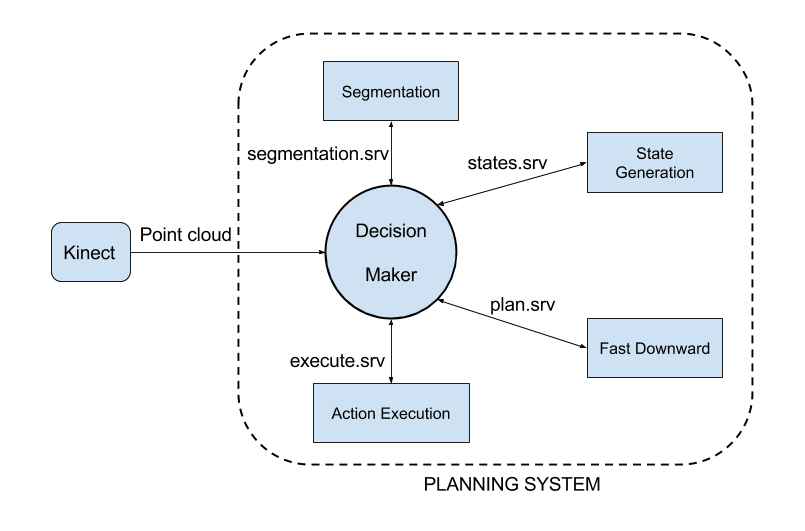
\includegraphics[width=14cm]{Img/software/Software_arquitecture.png}
\caption{Software architecture.}\label{fig:architecture}
\end{figure}


\paragraph{Simulation}
The implemented algorithm was first tested in simulation with Gazebo\citep{koenig2004design} before testing it in the real robot. A simple URDF model of the gripper (with no joints) was designed in order to simulate the pushing action. This model was not able to  simulate the grasp of an object, therefore the simulation of the grasping action was done in manner to remove the object in the simulation environment when the robot tried to grasp it. As debugging tool the RVIZ package\citep{RVIZ} has been used.  

In the simulation the real set up is accurately reproduced (Figure \ref{fig:sim_setup}). A simulation of the planning system is depicted in Figure \ref{fig:simulation} for a simple problem.
The first plan returned is: \ttt{(push\_dir1 o2) (push\_dir1 o0) (grasp o2) (grasp o1) (grasp o0)}. While the real executed plan is: \ttt{(push\_dir1 o2) (grasp o2) (push\_dir1 o0) (grasp o1) (grasp o0)}. The difference is only that it swaps the second action with the third one, this because the two plans have the same length and at every new frame the system replans again considering it as a problem uncorrelated to the previous one. 

After the algorithm was asserted to work as expected in simulation we moved to perform experiments with the real robot. 

\begin{figure}
\centering
\begin{subfigure}[h]{0.45\textwidth}
\centering
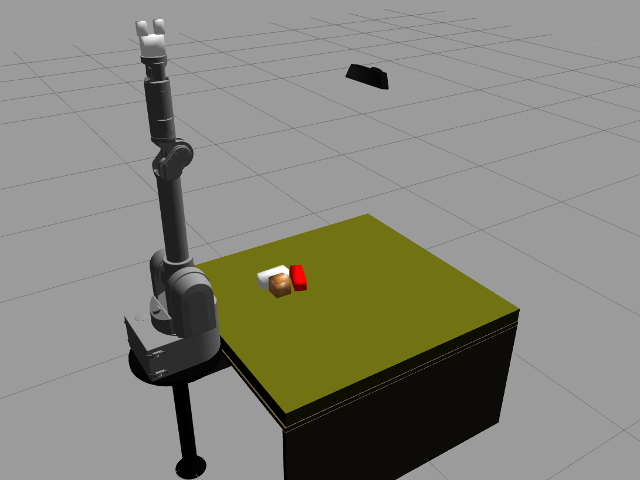
\includegraphics[width=6cm]{Img/simulation/setup_sim.png}
\caption{Simulation of the real set up}\label{fig:sim_setup}
\end{subfigure}
\begin{subfigure}[h]{0.45\textwidth}
\centering
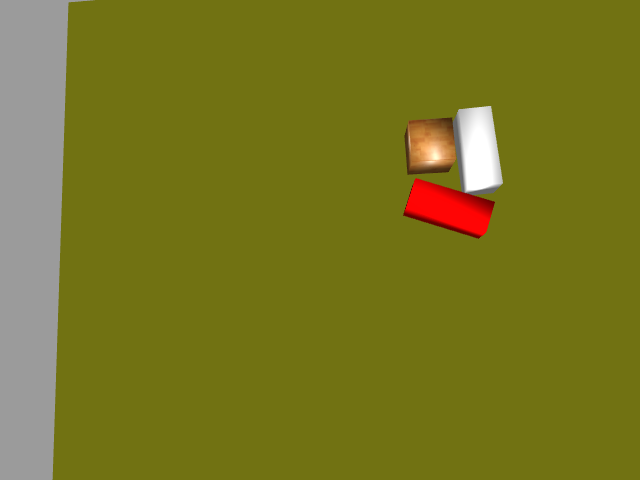
\includegraphics[width=6cm]{Img/simulation/image.png}
\caption{Kinect's view}
\label{fig:sim_kinect}
\end{subfigure}
\begin{subfigure}[h]{0.45\textwidth}
\centering
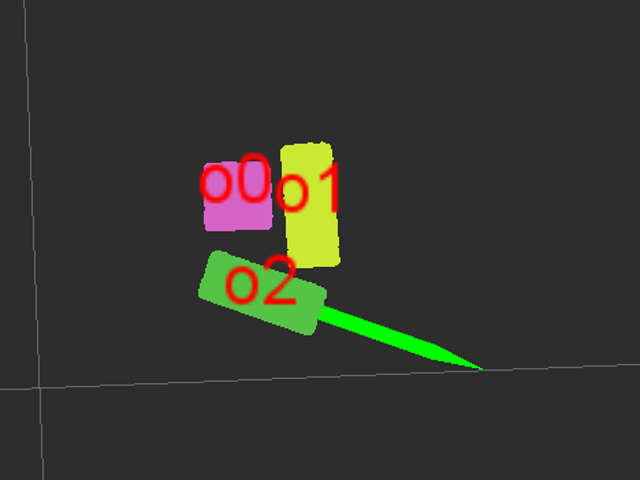
\includegraphics[width=6cm]{Img/simulation/action1.png}
\caption{Visualization in RVIZ of the objects and the action to execute (\ttt{(push\_dir1 o2)}).}
\label{fig:sim_rviz}
\end{subfigure}
\begin{subfigure}[h]{0.45\textwidth}
\centering
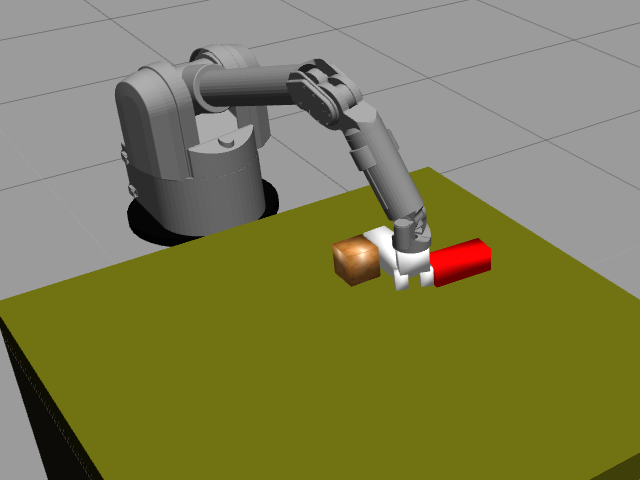
\includegraphics[width=6cm]{Img/simulation/pushing.png}
\caption{Execution of the first plan's action (\ttt{(push\_dir1 o2)}).}\label{fig:sim_push}
\end{subfigure}
\begin{subfigure}[h]{0.45\textwidth}
\centering
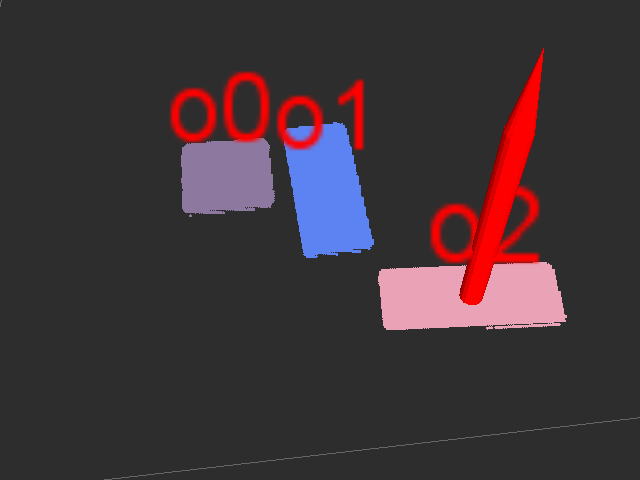
\includegraphics[width=6cm]{Img/simulation/action2.png}
\caption{Visualization in RVIZ of the objects and the action to execute (\ttt{(grasp o2)}).}\label{fig:action2}
\end{subfigure}
\begin{subfigure}[h]{0.45\textwidth}
\centering
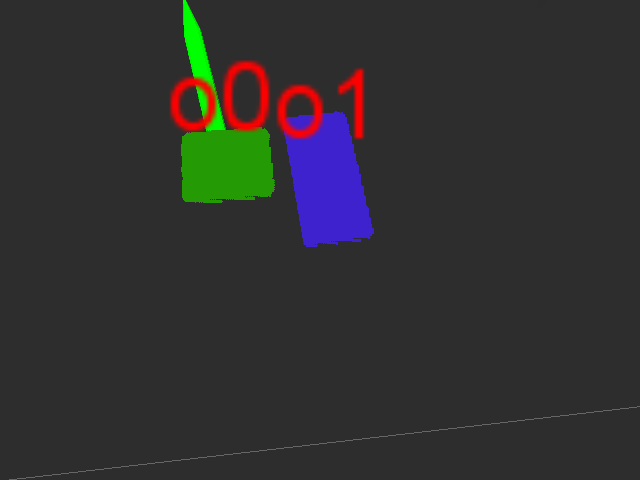
\includegraphics[width=6cm]{Img/simulation/action3.png}
\caption{Visualization in RVIZ of the objects and the action to execute (\ttt{(push\_dir1 o0)}).}\label{fig:action3}
\end{subfigure}
\caption{Simulation in Gazebo of a simple experiment.}\label{fig:simulation}
\end{figure}